% !TEX program = xelatex
% XeLaTeX source for the 5 x 8 inch edition -- Vietnamese translation.
\documentclass[10pt,twoside,openany]{book}

\usepackage{geometry}
\geometry{
  paperwidth=5in,
  paperheight=8in,
  top=0.7in,
  bottom=0.7in,
  inner=0.5in,
  outer=0.5in,
  headheight=10pt,
  headsep=20pt,
  footskip=25.2pt
}
\addtolength{\textheight}{-12pt}

\usepackage{fontspec}
\usepackage{xeCJK}
\usepackage{setspace}
\defaultfontfeatures{Ligatures=TeX}
\setmainfont[Path=fonts/]{SourceHanSerifCN-Regular.otf}
\setCJKmainfont[Path=fonts/]{SourceHanSerifCN-Regular.otf}
\setsansfont[Path=fonts/]{SourceHanSansCN-Medium.otf}
\setCJKsansfont[Path=fonts/]{SourceHanSansCN-Medium.otf}
\newfontfamily\SeparatorFont{lmroman10-regular.otf}
\xeCJKsetup{PunctStyle=plain}

\usepackage{fancyhdr}
\usepackage{xcolor}
\usepackage{pdfpages}
\usepackage[unicode=true,hidelinks]{hyperref}
\definecolor{PrimaryInk}{HTML}{161618}
\definecolor{SecondaryInk}{HTML}{5C5C62}
\color{PrimaryInk}
\hypersetup{
  pdftitle={Bạn gái tôi, Cảnh Điềm},
  pdfauthor={Justin Sun (孙宇晨)},
  pdfsubject={Bản dịch tiếng Việt -- 5 x 8 inch XeLaTeX edition}
}

% Body paragraphs begin flush with the text block.
\setlength{\parindent}{0pt}
\setlength{\parskip}{0pt}
\setlength{\topskip}{10pt}
\renewcommand{\baselinestretch}{1}
\clubpenalty=10000
\widowpenalty=10000
\displaywidowpenalty=10000
\brokenpenalty=10000
\raggedbottom

\fancypagestyle{bodyrunning}{
  \fancyhf{}
  \fancyhead[LO]{\sffamily\fontsize{8}{10}\selectfont\color{SecondaryInk}Bạn gái tôi, Cảnh Điềm}
  \fancyhead[RO]{\sffamily\fontsize{8}{10}\selectfont\color{SecondaryInk}\thepage}
  \fancyhead[LE]{\sffamily\fontsize{8}{10}\selectfont\color{SecondaryInk}\thepage}
  \fancyhead[RE]{\sffamily\fontsize{8}{10}\selectfont\color{SecondaryInk}Bạn gái tôi, Cảnh Điềm}
  \renewcommand{\headrulewidth}{0pt}
  \renewcommand{\footrulewidth}{0pt}
}

\fancypagestyle{bodyopening}{
  \fancyhf{}
  \fancyfoot[C]{\sffamily\fontsize{8}{10}\selectfont\color{SecondaryInk}\thepage}
  \renewcommand{\headrulewidth}{0pt}
  \renewcommand{\footrulewidth}{0pt}
}

\newcommand{\BodySingleLeading}{17.3076923}
\newcommand{\StoryParagraph}[2]{%
  \begingroup
  \rmfamily
  \setstretch{1.3}%
  \fontsize{9.5}{\BodySingleLeading}\selectfont
  #2\par
  \vspace{#1pt}
  \endgroup
}

\newcommand{\NarrativeBreak}{%
  \par\penalty10000
  \vspace{37.4pt}
  \noindent\hbox to \textwidth{\hfil\SeparatorFont\setstretch{1.3}\fontsize{9.5}{\BodySingleLeading}\selectfont\char"002D\kern0.12em\char"002D\kern0.12em\char"002D\hfil}\par
  \vspace{31.4pt}
  \penalty10000
}

\newcommand{\UnprintedPause}{%
  \par\penalty10000\vspace{22pt}\penalty10000
}

\begin{document}
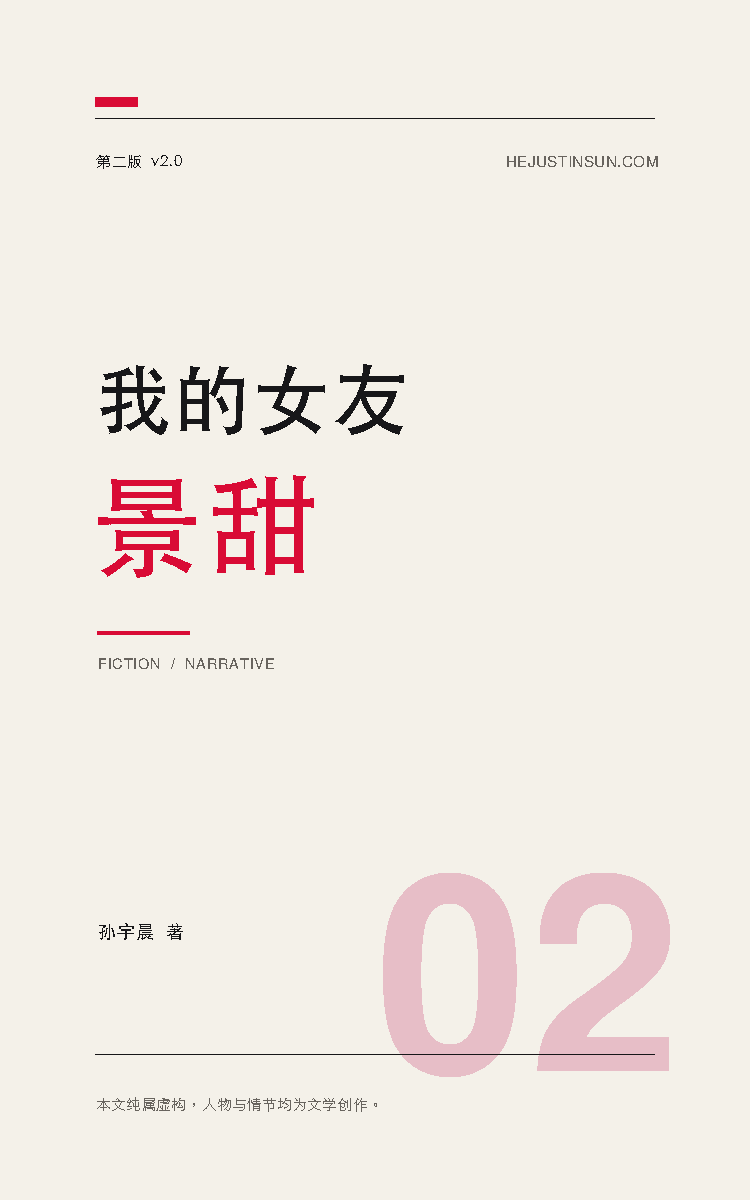
\includepdf[
  pages=1,
  fitpaper=true,
  noautoscale=true,
  pagecommand={\thispagestyle{empty}}
]{assets/cover.pdf}

% Half-title page for the Vietnamese edition.
\thispagestyle{empty}
\vspace*{0.9in}
\begin{center}
  {\rmfamily\fontsize{17}{22}\selectfont Bạn gái tôi, Cảnh Điềm}\\[10pt]
  {\sffamily\fontsize{8.5}{12}\selectfont\color{SecondaryInk}Justin Sun\ \ 孙宇晨}\\[26pt]
  {\sffamily\fontsize{8}{11}\selectfont\color{SecondaryInk}Nguyên tác 《我的女友景甜》}\\[3pt]
  {\sffamily\fontsize{8}{11}\selectfont\color{SecondaryInk}Bản dịch tiếng Việt}\\[26pt]
  {\sffamily\fontsize{8}{11}\selectfont\color{SecondaryInk}Tác phẩm hư cấu.}
\end{center}
\clearpage

\pagenumbering{arabic}
\setcounter{page}{1}
\pagestyle{bodyrunning}
\thispagestyle{bodyopening}
% Opening-page breathing room.
\vspace*{70.817pt}

\StoryParagraph{3}{Một tế bào trứng nặng ba phẩy năm microgam.}

\StoryParagraph{3}{Năm mươi triệu đô la tiền mặt nặng hai phẩy năm tấn.}

\StoryParagraph{3}{Trong cuộc gọi từ Montage Laguna Beach, thứ Cảnh Điềm đòi ở tôi là cái sau, thứ đem ra thế chấp là cái trước.}

\StoryParagraph{3}{Cô đến đó để lấy trứng. Đứa bé mang thai hộ dự kiến sinh năm 2027, nhanh chân thì còn kịp tuổi Ngọ. Chuyện này là cô chủ động đề nghị. Đến phòng khám rồi, cô nói không có năm mươi triệu thì không lấy.}

\UnprintedPause

\StoryParagraph{0}{Montage Laguna Beach nằm trên vách đá, bên dưới là Thái Bình Dương. Bao trọn một tầng, ba mươi ngày, một triệu đô, để cô được riêng tư. Cô ở tám ngày rồi đi.}

\StoryParagraph{0}{Hai mươi hai ngày còn lại, người dọn phòng vẫn lên đều đặn mỗi ngày. Trợ lý tôi kể, hôm đi trả chìa khóa có bắt gặp một lần: một người phụ nữ Mexico đẩy xe, vào từng phòng một, thay khăn, lau mặt bàn, giắt lại mép chăn, lùi ra khép cửa. Xong cả một tầng, hai tiếng.}

\StoryParagraph{0}{Trợ lý hỏi chị ta, không có ai ở, sao vẫn phải làm.}

\StoryParagraph{0}{Chị ta nói, trên sổ ghi là có người.}

\StoryParagraph{0}{Một cung điện Versailles đã mất hoàng hậu.}

\StoryParagraph{0}{Tôi chợt nhận ra, Cảnh Điềm thích thế. Cảnh Điềm thích một nơi chốn bỏ trống vì cô. Không có gì xảy ra cả.}

\StoryParagraph{3}{Bỏ trống cùng Montage Laguna Beach còn có một chiếc Gulfstream G700 đậu ngượng nghịu ở Van Nuys, tổ bay ngày nào cũng đến điểm danh như thường.}

\StoryParagraph{3}{Ngày thứ tám cô gọi cuộc điện thoại đó. Sau đó không ai gặp lại cô nữa.}

\NarrativeBreak

\StoryParagraph{0}{Năm 2007, đã có người đốt tiền cho cô rồi. Năm đó tôi vừa vào Đại học Bắc Kinh.}

\StoryParagraph{3}{Tất nhiên, người đốt tiền không phải tôi.}

\StoryParagraph{3}{Một cửa sổ QQ bật lên, gương mặt đại diện là cô. Ngay trên cái máy Lenovo IBM cũ đó, độ phân giải nhòe nhoẹt. Tôi lưu tấm ảnh lại.}

\StoryParagraph{3}{Tôi ngồi mạng trong ký túc xá Bắc Đại tiền phòng một nghìn tệ một năm, tìm được cô trên Xiaonei, gửi lời mời kết bạn. Xiaonei bắt điền một câu nhắn, tôi viết rồi xóa, xóa rồi viết, loay hoay chừng bốn mươi phút, cuối cùng gửi đi hai chữ “Chào bạn”.}

\StoryParagraph{3}{Cô không đồng ý.}

\StoryParagraph{3}{Có lẽ cô chưa từng dùng Xiaonei.}

\StoryParagraph{3}{Những năm về sau, làm việc gì tôi cũng nghĩ một câu hỏi: đến mức nào thì cô sẽ bấm đồng ý. Lúc có tỷ đầu tiên tôi đã nghĩ, lúc mười tỷ tôi cũng nghĩ.}

\StoryParagraph{3}{Về sau tôi không nghĩ nữa. Renren sập từ đời nào rồi.}

\StoryParagraph{3}{Tôi không gửi lời mời lần thứ hai.}

\StoryParagraph{3}{Năm 2011, Bắc Kinh lạnh. Tôi mua một cái áo phao, một trăm năm mươi tệ. Tôi nhớ cái giá đó, vì tôi đã do dự ba ngày.}

\StoryParagraph{3}{Cùng năm ấy cô đóng một bộ phim một trăm năm mươi triệu tệ, Chiến Quốc. Tôn Hồng Lôi, Ngô Trấn Vũ, Kim Hee-sun, Nakai Kiichi, Khương Vũ — cũng như Montage Laguna Beach và chiếc G700 mười chín năm sau — được mời tới để làm nền. Họ không biết vì sao mình có mặt ở đó, đã đến rồi thì phải có chuyện gì xảy ra chứ, nhưng chẳng có gì xảy ra cả.}

\StoryParagraph{3}{Rồi đến Trường Thành một trăm năm mươi triệu đô. Trương Nghệ Mưu, Lưu Đức Hoa, Matt Damon. Rồi đến Thành Long. Danh sách của vũ trụ Cảnh Điềm mỗi lúc một dài.}

\StoryParagraph{3}{Khi ấy tôi đã ở Mỹ, đi học, khởi nghiệp, càng ngày càng bận. Điều duy nhất không đổi là, cứ đổi một thiết bị, dù phiền đến đâu, tôi đều chép tấm ảnh QQ đó sang.}

\StoryParagraph{3}{Mười chín năm sau, trong danh sách có thêm tôi.}

\NarrativeBreak

\StoryParagraph{3}{Chúng tôi gặp nhau lần đầu ở khách sạn Rosewood. Tôi vẫn tưởng hôm gặp cô mình sẽ hồi hộp.}

\StoryParagraph{3}{Không hề.}

\StoryParagraph{3}{Cô gầy hơn trong ảnh, mặc rất xuề xòa, tựa vào sofa. Tôi nhìn cô, bỗng dưng không nhớ nổi rốt cuộc mình đã chờ cái gì.}

\StoryParagraph{3}{Tôi dẫn cô đi xem quả chuối của Cattelan. Cô nhìn rất lâu, hỏi tôi, cái này bao nhiêu tiền.}

\StoryParagraph{3}{Sáu triệu hai trăm nghìn đô.}

\StoryParagraph{3}{Cô nói, thế nó thối thì sao.}

\StoryParagraph{3}{Tôi im lặng. Cô nói, thôi kệ, mình đi xem phim đi.}

\StoryParagraph{3}{Tôi nói ừ.}

\StoryParagraph{3}{Cô nói trong phòng chiếu, ngoài hai đứa mình ra, không được có ai hết.}

\StoryParagraph{3}{Tôi nói ừ.}

\StoryParagraph{3}{Tôi ra ngoài gọi một cuộc. Lúc quay lại cô vẫn đứng trước quả chuối đó.}

\StoryParagraph{3}{Bộ phim là Zootopia 2.}

\StoryParagraph{3}{Phòng chiếu chỉ có hai người — cảnh này thường chỉ dùng khi Ban Tuyên giáo Trung ương duyệt phim.}

\StoryParagraph{3}{Tôi bảo trợ lý mua sạch mọi ghế trong rạp.}

\StoryParagraph{3}{Tôi từng đọc mấy bài phê phán chuyện mua doanh thu ảo, nói vé bán hết mà chỉ có hai người xem. Giờ tôi mới hiểu, có lẽ không hẳn vì doanh thu.}

\StoryParagraph{3}{Mua hết ghế thì không khó, phiền là mấy tấm vé đã bán ra. Trợ lý và vệ sĩ đến trước cửa rạp, gặp khán giả đã mua vé thì dúi tiền mặt vào tay.}

\StoryParagraph{3}{Một đôi vợ chồng dắt con đến, đứa bé đã giơ cao bịch bỏng ngô ngay trước cửa.}

\StoryParagraph{3}{Trợ lý đưa một xấp tiền, đứa bé không hiểu vì sao không được vào, người lớn cầm tiền, cảm ơn, không hỏi gì cả, đi về.}

\StoryParagraph{3}{Hôm đó có hai mươi sáu người nhận tiền.}

\StoryParagraph{3}{Xem xong cô đổi ảnh đại diện WeChat thành cảnh sát thỏ Judy.}

\StoryParagraph{3}{Buổi tối tôi đưa tay bóp ngực cô, bị cô gạt ra.}

\StoryParagraph{3}{Tôi tưởng cô không muốn. Tôi rụt tay về, định nói gì đó.}

\StoryParagraph{3}{Cô không nói gì. Cô ngồi dậy, lục trong túi ra một cái bọc nhỏ, kéo khóa, bên trong là một dãy đồ, trông như một bộ dụng cụ rất nhỏ.}

\StoryParagraph{3}{Cô nói, móng tay anh cào em đau.}

\StoryParagraph{3}{Tôi nhìn thử. Xưa nay tôi vẫn lấy bấm móng tay cắt qua loa, mép còn nhọn, bình thường chẳng thấy gì.}

\StoryParagraph{3}{Cô nói, lại đây.}

\StoryParagraph{3}{Cô đặt tay tôi lên đùi cô, dũa từng ngón một.}

\StoryParagraph{3}{Đầu tiên là mặt ráp, dũa xong đổi mặt, rồi lại đổi mặt nữa. Dũa một lúc lại giơ lên soi vào đèn, rồi dũa tiếp.}

\StoryParagraph{3}{Tôi hỏi cái này phải dũa bao lâu.}

\StoryParagraph{3}{Cô nói, dũa đến khi nào không cào người nữa thì thôi.}

\StoryParagraph{3}{Mười ngón tay, cô mất gần một tiếng.}

\StoryParagraph{3}{Giữa chừng cô dạy tôi, mặt này dũa dáng, mặt này đánh bóng, mặt cuối cùng đừng chà đi chà lại, phải miết theo một chiều.}

\StoryParagraph{3}{Tôi nói vâng.}

\StoryParagraph{3}{Dũa xong cô lật tay tôi lên xem, sờ một cái.}

\StoryParagraph{3}{Cô nói, được rồi.}

\StoryParagraph{3}{Sờ đi, muốn sờ đâu cũng được.}

\StoryParagraph{3}{Giữa chừng cô có nói một câu. Cô nói, mai này em không còn nữa, sẽ chẳng còn ai đánh bóng móng tay cho anh.}

\StoryParagraph{3}{Tôi cười một cái, không nói gì.}

\StoryParagraph{0}{Quen cô được ba tháng, tôi cho người làm một tập tài liệu. Các dự án của cô những năm đó, đối tác, cổ phần công ty, Cảnh Quốc Khánh, Điền Tâm Ái, mấy tài khoản liên quan, căn nhà thuê ở Bắc Kinh, căn nhà mua ở Thượng Hải, và một số thứ khác. Một tuần là xong, tất cả hơn bốn mươi trang. Còn có mấy chuyện trai gái, tôi thấy đó là phần không quan trọng nhất.}

\StoryParagraph{0}{Trong đó có vài chuyện về sau cô kể lại cho tôi, kể khác với những gì viết trên giấy. Tôi không nói gì.}

\StoryParagraph{0}{Có vài chuyện cô không bao giờ kể. Tôi cũng không hỏi.}

\StoryParagraph{0}{Tôi tin tất cả những gì cô nói.}

\StoryParagraph{0}{Tập tài liệu đó tôi giữ, giữ đến tận bây giờ.}

\StoryParagraph{3}{Nhưng tôi không tin lấy một chữ.}

\NarrativeBreak

\StoryParagraph{3}{Cô nói, Hồng Kông đông người quá, sẽ bị nhận ra, mình đi đâu đó chơi đi.}

\StoryParagraph{3}{Tôi nói ừ.}

\StoryParagraph{3}{Cô chỉ tay vào Tenerife trên bản đồ.}

\StoryParagraph{3}{Tôi nói ừ.}

\StoryParagraph{3}{Tôi ra ngoài gọi một cuộc, quay vào mới biết chỗ đó nằm giữa Đại Tây Dương, ngoài khơi tây bắc châu Phi. Trưa hôm sau, đoàn ba mươi người chúng tôi lên đường, chiếc A330 đã chờ sẵn ở sân bay.}

\StoryParagraph{3}{Trong buồng ngủ trên máy bay cô hỏi tôi, tên em có hay không.}

\StoryParagraph{3}{Tôi nói hay.}

\StoryParagraph{3}{Cô nói, là họ của bố em ghép với họ của mẹ em đấy, có khéo không.}

\StoryParagraph{3}{Tôi nói ngày đầu tiên anh đã nhớ rồi.}

\StoryParagraph{3}{Cô ôm tôi, nói, sau này đừng gọi em là Cảnh Điềm nữa, gọi em là mẹ đi.}

\StoryParagraph{3}{Vâng, mẹ.}

\StoryParagraph{3}{Hạ cánh xong cơ trưởng đến báo: sếp ơi, lúc đầu trên đảo không cho hạ, họ chưa thấy máy bay riêng nào to thế này.}

\StoryParagraph{3}{Trên đảo vẫn luật cũ, xung quanh không được có ai. Trợ lý đi lo, không ai hỏi vì sao, lần này tôi không hỏi là bao nhiêu người.}

\StoryParagraph{3}{Ritz-Carlton nhìn thẳng ra Đại Tây Dương, cửa kính quá lớn. Mẹ ngủ không chịu được một tia sáng nào. Trợ lý lấy băng keo đen dán kín cả căn phòng, bên ngoài sáng như ban ngày, bên trong tối như phòng biệt giam. Băng keo phơi nắng là bong, ngày nào cũng phải dán lại.}

\StoryParagraph{3}{Trợ lý cả thảy mười một người, sáu rưỡi sáng có mặt, đợi chúng tôi ngủ rồi mới về. Dán băng keo là hai cô gái, một người lo khung cửa, một người lo đèn báo của điều hòa và ổ điện, dán xong kiểm tra lại ba lượt. Băng keo mua ba mươi cuộn, sau bổ sung thêm hai mươi. Hai cô phát hiện dán sau ba giờ chiều là dễ bong nhất, vì lúc đó kính nóng nhất, về sau đổi sang dán buổi sáng. Chuyện này không ai dạy họ, họ tự mò ra. Họ bàn với nhau, như bàn về một nghề thủ công.}

\StoryParagraph{3}{Cô biết tên hai cô gái đó. Tôi thì không.}

\StoryParagraph{3}{Chúng tôi dừng xe bên đường ở Vườn quốc gia Teide ngắm hoàng hôn, trợ lý khiêng hoa hồng từ trên xe xuống, khui sâm banh.}

\StoryParagraph{3}{Mẹ nhìn biển mây, nói, đẹp quá. Nhưng không bằng hoàng hôn ở Đức Lệnh Cáp, Thanh Hải.}

\StoryParagraph{3}{Tôi là người Thanh Hải.}

\StoryParagraph{3}{Tôi không nói gì.}

\StoryParagraph{3}{Đêm chúng tôi lên đỉnh núi ngắm sao, mặc áo bông vẫn lạnh.}

\StoryParagraph{3}{Mẹ nói, ước một điều đi.}

\StoryParagraph{3}{Tôi hỏi, em ước gì.}

\StoryParagraph{3}{Mẹ nói, không nói cho anh biết đâu.}

\StoryParagraph{3}{Mẹ nói, đẹp quá. Nhưng lạnh quá, mình đi Maldives đi.}

\StoryParagraph{3}{Tôi nói, ừ thì đi.}

\StoryParagraph{3}{Tenerife âm mười lăm độ, Maldives hai mươi bảy độ, đường chim bay chín nghìn năm trăm cây số, bay mười một tiếng. Có điều sân bay Maldives nhỏ quá, máy bay thân rộng của chúng tôi giữa chừng phải đổi sang máy bay nhỏ.}

\StoryParagraph{3}{Mẹ nói, máy bay nhỏ ồn quá. Vẫn là máy bay to hơn.}

\StoryParagraph{3}{Trong buồng ngủ trên chuyến bay đi Maldives, mẹ nói với tôi, điều cô ước là có với tôi một đứa con. Bắt buộc phải mang thai hộ.}

\StoryParagraph{3}{Tôi chưa từng hỏi vì sao. Tôi tưởng cô sợ đau.}

\StoryParagraph{3}{Giữa chừng mẹ bỗng ngồi bật dậy tìm điện thoại, nối Starlink, nói hỏng rồi.}

\StoryParagraph{3}{Tôi hỏi sao thế.}

\StoryParagraph{3}{Cô nói, có người dọa em, hỏi ba ngày nay rồi, em vẫn chưa trả lời.}

\StoryParagraph{3}{Tôi nói bao nhiêu.}

\StoryParagraph{3}{Cô nói không cần anh lo.}

\StoryParagraph{3}{Cô gõ rất lâu, xóa rồi sửa, sửa rồi xóa. Gõ xong úp điện thoại xuống đùi, một lát lại lật lên xem.}

\StoryParagraph{3}{Tôi hỏi người đó là ai.}

\StoryParagraph{0}{Cô nói, người từng làm với em, kế toán, vào tù, gánh tội.}

\StoryParagraph{3}{Ra tù không còn đường sống, nhất định phải tìm em.}

\StoryParagraph{3}{Tôi nói, hay báo công an bắt quách đi.}

\StoryParagraph{3}{Cô liếc tôi một cái. Anh không hiểu đâu.}

\StoryParagraph{3}{Tôi hỏi em đưa chưa.}

\StoryParagraph{3}{Cô nói đưa rồi.}

\StoryParagraph{3}{Bao nhiêu.}

\StoryParagraph{3}{Tám mươi nghìn.}

\StoryParagraph{3}{Tôi nói, chuyện này mà cũng phải nghĩ ba ngày.}

\StoryParagraph{3}{Cô không nói gì.}

\StoryParagraph{3}{Thời gian còn lại của ngày hôm đó cô gần như không nói gì nữa. Hạ cánh rồi mới ngủ.}

\StoryParagraph{0}{Đến Soneva Jani sớm nhất là vali của mẹ. Hành lý ba mươi người, máy bay nhỏ chở không hết, phải chia làm ba chuyến. Mẹ chỉ có một cái vali, đi riêng một chuyến, cô nói không muốn để chung với đồ người khác.}

\StoryParagraph{0}{Soneva Jani nổi tiếng với câu no news, no shoes, mẹ yên tâm.}

\StoryParagraph{3}{Quản gia khách sạn, vệ sĩ, trợ lý, cả thảy hai mươi sáu người, còn thêm hai người điều khiển flycam bám theo từ xa. Đám trợ lý lại bắt đầu dán băng keo, đèn điều hòa, đèn ổ điện, hết lượt này đến lượt khác.}

\StoryParagraph{0}{Buổi tối chúng tôi trao đổi người yêu cũ của nhau như trao mật hiệu, như hai vương triều đối chiếu niên hiệu. Mẹ không muốn có bất kỳ sai sót nào, có điều mẹ có một từ cấm kỵ: không được nhắc đến vận động viên kia.}

\StoryParagraph{0}{Tôi không nhắc, dù tôi biết hình xăm trên lưng mẹ là vì vận động viên kia mà xăm.}

\StoryParagraph{3}{Chắc tại nó to quá nên xóa không được.}

\StoryParagraph{0}{Cô nói, giờ mình là người một nhà rồi. Bố mẹ em nuôi em lớn thế này không dễ, anh phải có sính lễ.}

\StoryParagraph{0}{Tôi nói ừ.}

\StoryParagraph{0}{Cô đọc hai cái tên, Cảnh Quốc Khánh, Điền Tâm Ái, và hai số tài khoản.}

\StoryParagraph{0}{Ba mươi triệu, tệ.}

\StoryParagraph{0}{Tôi chuyển. Hai cái tên đó, lần đầu tiên tôi nhìn thấy là trong hơn bốn mươi trang kia.}

\StoryParagraph{3}{Một lát sau, cô đưa điện thoại cho tôi xem. Điền Tâm Ái nhắn lại hai chữ: Nhận rồi.}

\StoryParagraph{0}{Có lần mẹ nói, anh biết lúc em đòi mấy thứ đó em nghĩ gì không.}

\StoryParagraph{0}{Tôi nói nghĩ gì.}

\StoryParagraph{0}{Cô nói, em nghĩ, không biết có lần nào anh sẽ nói không.}

\StoryParagraph{0}{Tôi nói không có đâu.}

\StoryParagraph{0}{Cô nói, thế thì chán chết.}

\StoryParagraph{3}{Tôi nghĩ, còn gì mà tôi làm không được nữa đâu?}

\StoryParagraph{0}{Lúc quá rảnh, tôi mở tấm ảnh QQ năm 2007 ra nghịch, định chép sang máy mới. Mẹ ghé đầu sang: anh giấu em lưu ảnh đàn bà khác à, ai đây.}

\StoryParagraph{0}{Tôi im lặng. Không nói gì cả.}

\StoryParagraph{0}{Cô thấy ảnh nhòe quá, bèn quay đi làm việc khác.}

\StoryParagraph{0}{Đêm đó tôi xóa tấm ảnh.}

\StoryParagraph{3}{Hôm sau tôi lại lục trong máy cũ tìm về.}

\StoryParagraph{0}{Mẹ cũng lướt điện thoại không ngừng, tôi hỏi em xem gì đấy.}

\StoryParagraph{0}{Cô nói không có gì, mấy chuyện vớ vẩn tranh vị trí thôi.}

\StoryParagraph{0}{Tranh vị trí — một bộ phim chỉ có một ngôi sao được đứng đầu. Nam chính nữ chính cũng chỉ một người được đứng đầu.}

\StoryParagraph{0}{Tôi nói chán nhỉ.}

\StoryParagraph{0}{Cô nói, ừ. Khó hơn nữa là, có khi đóng vợ chồng, vào đoàn bốn năm chục ngày, thường thì đóng với một người đàn ông, tối làm tình, ngày còn phải tranh vị trí.}

\StoryParagraph{0}{Tôi nói phản nhân tính quá.}

\StoryParagraph{0}{Cô nói ừ.}

\StoryParagraph{0}{Có điều đóng xong rồi, trước đó làm tình bao nhiêu lần cũng coi như chưa có gì xảy ra.}

\StoryParagraph{3}{Rồi cô lại xem tiếp nửa tiếng.}

\StoryParagraph{0}{Ngày 2 tháng 1 năm 2026, ở Soneva Jani, năm mới, tôi cầu hôn mẹ.}

\StoryParagraph{0}{Quyết định là sáng ngày 1 tháng 1. Nhẫn ở Hồng Kông. Trên đảo không có chỗ nào bán nhẫn, trợ lý đi thủy phi cơ ra Malé, chiều về, nhẫn đựng trong một cái phong bì của khách sạn.}

\StoryParagraph{0}{Mẹ nói, nhẫn kim cương nhỏ quá.}

\StoryParagraph{0}{Mẹ nói, không sao, sau này bù cái to.}

\StoryParagraph{0}{À, anh sang Bắc Kinh được không?}

\StoryParagraph{0}{Tôi im lặng.}

\StoryParagraph{0}{Cô tưởng tôi không muốn đi.}

\StoryParagraph{0}{Mẹ nói, sao anh đối với em tốt thế.}

\StoryParagraph{0}{Tôi nói vì anh thích em.}

\StoryParagraph{0}{Cô nói, thế trước kia anh cũng đối với người khác như vậy à.}

\StoryParagraph{0}{Tôi nói không.}

\StoryParagraph{3}{Cô cười một cái, không nói gì.}

\StoryParagraph{0}{Có hôm tôi dậy sớm, cô không có trên giường.}

\StoryParagraph{0}{Tôi ra ngoài tìm, cô ngồi ngoài ban công, quay mặt ra biển, cả mặt biển đen kịt. Không bật đèn, trời chưa sáng.}

\StoryParagraph{0}{Tôi hỏi sao dậy sớm thế.}

\StoryParagraph{0}{Cô nói, em đang tính ngày.}

\StoryParagraph{0}{Tôi hỏi tính gì.}

\StoryParagraph{0}{Cô nói, anh vào ngủ tiếp đi.}

\StoryParagraph{0}{Tôi ngồi cạnh cô một lúc, không biết nói gì. Sau tôi vào ngủ tiếp.}

\StoryParagraph{3}{Lúc tôi tỉnh lại thì cô đã trang điểm xong.}

\StoryParagraph{0}{Ở Maldives mười bốn ngày, không một ai nhận ra cô.}

\StoryParagraph{0}{Tối ngày thứ mười ba ở nhà hàng, cô bỏ kính râm ra. Một lát sau, mũ cũng bỏ, đặt lên bàn. Cô cứ thế ngồi hết một bữa. Bàn bên cạnh là một đôi vợ chồng già người Đức, phục vụ là người Sri Lanka, không ai nhìn cô đến lần thứ hai.}

\StoryParagraph{0}{Ăn xong cô đội mũ lại.}

\StoryParagraph{0}{Mẹ nói, mình về đi.}

\StoryParagraph{0}{Tôi nói chưa ở đủ mà.}

\StoryParagraph{3}{Cô nói, yên tĩnh quá.}

\UnprintedPause

\StoryParagraph{0}{Về Hồng Kông, mẹ gặp bố mẹ tôi.}

\StoryParagraph{0}{Ngay tối hôm đó cô nói, nhà cần chuẩn bị cho hai bên gặp mặt và lo đám cưới, lo liệu càng nhiều càng tốt. Vẫn là Cảnh Quốc Khánh và Điền Tâm Ái.}

\StoryParagraph{0}{Tôi không hỏi vì sao.}

\StoryParagraph{0}{Tôi nói một ngày một thẻ, hạn mức một triệu.}

\StoryParagraph{0}{Mẹ nói chậm quá.}

\StoryParagraph{0}{Chuyển năm thẻ.}

\StoryParagraph{0}{Năm cái thẻ, hai số tài khoản, chuyển luân phiên. Chuyển đến thẻ thứ ba, tôi do dự một chút. Rồi tôi vẫn chuyển hết.}

\StoryParagraph{3}{Mẹ nói, hiệu suất thấp quá.}

\StoryParagraph{0}{Tôi nói, Tết đón bố mẹ hai bên sang Hồng Kông ăn Tết chung đi.}

\StoryParagraph{0}{Mẹ nói, năm nay đã định ăn Tết ở Hải Nam rồi. Sang năm vậy.}

\StoryParagraph{0}{Tết, Cảng Victoria bắn pháo hoa, một triệu người kéo đến. Không có cô.}

\StoryParagraph{0}{Ba giờ sáng, tôi đưa bố mẹ về.}

\StoryParagraph{0}{Đường rất vắng, đèn đỏ không một chiếc xe nào chờ, tôi vẫn dừng.}

\StoryParagraph{0}{Mẹ nói tạm thời chưa gặp, sắp đi Los Angeles lấy trứng rồi. Việc trong tay phải xử lý xong đã.}

\StoryParagraph{0}{Mẹ lại hỏi, sang Bắc Kinh được không?}

\StoryParagraph{0}{Tôi im lặng.}

\StoryParagraph{3}{Cô không nói ở Bắc Kinh có gì. Tôi cũng không hỏi.}

\StoryParagraph{0}{Mẹ nói, ở Hồng Kông nhất định phải mua một căn nhà, đứng tên cô.}

\StoryParagraph{0}{Tôi nói, ừ thì mua.}

\StoryParagraph{3}{Lễ Tình nhân cũng không gặp.}

\StoryParagraph{0}{Có lần cô nói qua điện thoại, sáng nay em bị lấy tám ống máu.}

\StoryParagraph{0}{Tôi nói nhiều thế.}

\StoryParagraph{0}{Cô nói cũng bình thường.}

\StoryParagraph{0}{Tôi nói vất vả rồi.}

\StoryParagraph{0}{Rồi chúng tôi nói sang chuyện khác.}

\StoryParagraph{0}{Về sau tôi mới biết, kiểu lấy máu đó phải nhịn ăn, phải làm vào ngày thứ hai hoặc thứ ba của chu kỳ, sai ngày là hỏng. Sáng hôm đó chắc khoảng sáu giờ cô đã ra khỏi nhà, mùa đông Bắc Kinh, trời còn chưa sáng. Về sau các lần khám mỗi lúc một nhiều. Tôi biết chuyện này là vì trong bảng thanh toán tổng hợp hằng tháng của trợ lý có thêm một mục. Lần đầu xuất hiện là năm ngoái, số tiền không lớn, mấy nghìn tệ. Sau tháng nào cũng có, có tháng hai ba khoản. Tôi duyệt rất nhanh. Những khoản như thế không cần tôi xem chi tiết. Mãi sau tôi mới biết đó là lấy máu, xét nghiệm sáu chỉ số nội tiết, siêu âm, AMH. Để xem cô còn bao nhiêu dự trữ, lấy ra được mấy quả, có đáng đi tiếp hay không.}

\StoryParagraph{0}{Tất cả đều làm ở Bắc Kinh.}

\StoryParagraph{3}{Tôi không biết là bệnh viện nào. Tôi cũng không biết cô tự đi, hay có ai đi cùng.}

\StoryParagraph{0}{Ngày 25 tháng 2 cô đáp xuống Hồng Kông.}

\StoryParagraph{0}{Cô nói không đi Los Angeles nữa, trừ khi được xem nhà ở Hồng Kông trước.}

\StoryParagraph{0}{Tôi gửi cho cô hơn chục căn đã xem suốt nửa năm qua. Cô chê xấu hết. Hơn chục căn đó tôi chưa đến căn nào, là trợ lý mất nửa năm đi lọc từng căn, trợ lý gửi cho tôi, tôi gửi cho cô. Có một căn ở Mid-Levels, trong video nhìn thấy được Cảng Victoria, quay lúc chạng vạng. Có một khoảnh khắc máy rung một cái, quay được bóng của người quay hắt lên tường. Tôi nhìn cái bóng đó mà nghĩ, người này là ai, hôm nay anh ta đã đi bao nhiêu đường, xem bao nhiêu căn nhà, anh ta có biết căn nhà này là xem cho ai không.}

\StoryParagraph{3}{Thời gian gấp quá, cuối cùng cô vẫn lên chiếc G700 đi Los Angeles, ngày 28 tháng 2 bay đến Montage Laguna Beach.}

\NarrativeBreak

\StoryParagraph{0}{Ngày thứ tám mẹ gọi điện. Bên đó là buổi chiều, bên tôi là rạng sáng.}

\StoryParagraph{0}{Cô nói, năm mươi triệu, đô la.}

\StoryParagraph{0}{Tôi nói, để anh nghĩ đã.}

\StoryParagraph{0}{Cô không nói gì. Tôi nghe thấy tiếng biển bên đó.}

\StoryParagraph{0}{Một lát sau cô nói, được.}

\StoryParagraph{0}{Cô cúp máy.}

\StoryParagraph{3}{Từ ngày quen cô, tôi chưa từng nói với cô câu “để anh nghĩ đã”.}

\StoryParagraph{0}{Tôi dùng Claude Code đọc API chạy một lượt toàn bộ tài sản tiền mặt, kết luận là chuyện này không ảnh hưởng gì đến tôi. Tôi đối chiếu lại một lần nữa. Tôi gõ câu hỏi vào Claude Code, Claude nói: đừng đưa năm mươi triệu đô đó cho cô ấy.}

\StoryParagraph{3}{Tôi hỏi, cô ấy không còn yêu tôi nữa sao?}

\StoryParagraph{3}{Claude nói, về tình yêu, tôi không quan tâm, cũng không hiểu. Nhưng anh không thể đưa năm mươi triệu đô đó cho cô ấy.}

\StoryParagraph{3}{Xưa nay tôi chưa từng từ chối cô, không phải vì hào phóng, mà vì sợ. Sợ câu trả lời của giây tiếp theo.}

\StoryParagraph{0}{Còn bây giờ đã có người nói thay tôi.}

\StoryParagraph{0}{Tôi nhìn dòng chữ đó rất lâu. Thứ làm tôi rợn người không phải là nó thông minh, mà là Claude không do dự một chút nào.}

\StoryParagraph{0}{Nó không thấy khó xử.}

\StoryParagraph{0}{Lúc đó tôi nghĩ, đây chắc là một thứ gì đó cao hơn. Con người không làm được như vậy.}

\StoryParagraph{3}{Cô ấy không còn yêu tôi nữa sao.}

\StoryParagraph{3}{Hôm sau cô gọi lại.}

\StoryParagraph{3}{Mẹ nói, biển rộng lắm.}

\StoryParagraph{3}{Tôi nói thế à.}

\StoryParagraph{3}{Cô nói, tầng này rộng quá, có tiếng vọng. Sáng có người lên dọn, em trốn trong nhà vệ sinh đợi họ đi.}

\StoryParagraph{3}{Tôi nói có thể không cho họ lên.}

\StoryParagraph{3}{Cô nói không cần.}

\StoryParagraph{3}{Cô nói, phòng khám hỏi em, bao giờ bố của đứa bé đến.}

\StoryParagraph{3}{Tôi nói anh cho người sang được.}

\StoryParagraph{3}{Cô nói, không cần.}

\StoryParagraph{3}{Rồi cô nói, nghĩ xong chưa.}

\StoryParagraph{3}{Tôi không nói gì. Không phải đang nghĩ — tôi chẳng nghĩ gì cả. Trong điện thoại bên cô có biển, bên tôi là Cảng Victoria, hai bên đều không ai nói gì. Tôi đếm, mười một giây.}

\StoryParagraph{3}{Cảnh Điềm nói, được.}

\StoryParagraph{3}{Cảnh Điềm nói, em biết rồi.}

\StoryParagraph{3}{Cô cúp máy.}

\StoryParagraph{3}{Về sau tôi đã nhớ lại vô số lần, hai ngày đó ngoài năm mươi triệu cô còn nói gì. Biển rộng lắm, tầng này rộng quá, cô trốn trong nhà vệ sinh. Chỉ có thế, tôi nhớ hết, không sai một chữ. Thứ tôi không nhớ nổi là giọng cô — lúc cô nói “em biết rồi”, là giọng gì.}

\StoryParagraph{0}{Tôi không nhớ ra. Về sau tôi thôi không nhớ nữa.}

\StoryParagraph{0}{Tôi đặt điện thoại lên tủ đầu giường, úp màn hình xuống. Rồi tôi làm một việc mà đến giờ vẫn không hiểu vì sao: tôi đặt tay lên ngực, đếm nhịp.}

\StoryParagraph{0}{Tim đập rất đều.}

\StoryParagraph{0}{Tôi đếm lại lần nữa, vẫn rất đều. Một phút sáu mươi mấy nhịp, không khác gì ngày thường. Tôi ngồi đó, tay ấn lên ngực mình, như một bác sĩ đang khám cho người khác.}

\StoryParagraph{3}{Tôi nghĩ, hóa ra là thế.}

\StoryParagraph{0}{Thời gian còn lại của ngày hôm đó tôi không làm gì cả. Tôi ở trong phòng từ lúc trời tối đến lúc trời sáng, nhìn Cảng Victoria từ màu xanh chuyển sang xám rồi sang đen. Sáu giờ sáng, bên kia cảng những tòa tài chính lần lượt bật đèn. Giữa chừng trợ lý có gõ cửa một lần, hỏi bữa tối sắp xếp thế nào, tôi nói thôi khỏi.}

\StoryParagraph{3}{Tôi không khóc. Tôi cứ chờ mình khóc.}

\NarrativeBreak

\StoryParagraph{0}{Sau này trợ lý quyết toán với tôi, trong đó còn một mục là tiền đền cho khách sạn ở Tenerife. Sau khi chúng tôi đi, băng keo vẫn được dán thêm mấy ngày nữa, không ai bảo họ là thôi đừng dán. Khách sạn nói dán lâu quá, nhiều lần quá, vết keo trên khung cửa không tẩy được, phải thay nguyên tấm kính đó.}

\StoryParagraph{0}{Tôi nói duyệt.}

\StoryParagraph{3}{Tấm kính đó quay ra Đại Tây Dương.}

\StoryParagraph{0}{Trong hóa đơn, mục nhiên liệu máy bay còn đắt hơn cả tầng lầu ở Montage. Tôi hỏi thử. Trợ lý nói, A330 thiết kế cho hai trăm người, chúng ta chỉ có ba mươi người, nhẹ quá, cân bằng lúc cất cánh không đúng. Nên lần nào cũng phải bơm thêm dầu, bơm đến khi đủ nặng. Đến nơi rồi, chỗ dầu bơm thêm đó cũng không giữ lại được, phải xả bỏ.}

\StoryParagraph{0}{Tôi nói, lần nào cũng thế à?}

\StoryParagraph{3}{Anh ta nói, lần nào cũng thế.}

\StoryParagraph{0}{Còn một cái thùng phòng khám ở Los Angeles gửi trả về. Thuốc kích trứng tám ngày, phải bảo quản lạnh, không mở một ống nào.}

\StoryParagraph{3}{Còn tiền đặt cọc cho công ty mang thai hộ, hai trăm nghìn đô, không hoàn lại. Người mang thai hộ đã chốt từ tháng Một, người California, ba mươi tư tuổi, đã sinh hai lần. Trong hồ sơ có ảnh của cô ấy, tôi chưa xem. Cô ấy đã sẵn sàng từ tháng Một.}

\StoryParagraph{3}{Cảnh Điềm đi rồi, tôi lôi tấm ảnh năm 2007 ra xem một lần. Mười chín năm, thiết bị càng ngày càng nhiều điểm ảnh, mà tấm ảnh này thì như càng ngày càng ít, mặt nhòe hết. Tôi phóng to nhìn rất lâu, muốn tìm xem cô hồi đó và cô về sau khác nhau ở chỗ nào. Không tìm ra chỗ nào cả. Vì tấm ảnh đó vốn dĩ đã không nhìn rõ.}

\StoryParagraph{0}{Có hôm tôi lấy bấm móng tay cắt móng, cắt xong sờ thử, vẫn nhọn.}

\StoryParagraph{0}{Tôi nhớ ra trong ngăn kéo còn cái đồ đó, cô để lại.}

\StoryParagraph{0}{Tôi lấy ra dũa hai cái, không đúng. Cô từng nói phải miết theo một chiều, tôi quên mất là chiều nào.}

\StoryParagraph{0}{Tôi cất nó lại vào ngăn kéo.}

\StoryParagraph{3}{Móng tay tôi giờ vẫn cào người.}

\StoryParagraph{0}{Có buổi sáng điện thoại hiện một lời nhắc, là trợ lý đặt lịch từ năm ngoái: ba tháng trước ngày dự sinh, chuẩn bị phòng.}

\StoryParagraph{3}{Tôi gạt nó đi.}

\StoryParagraph{0}{Từ khi cô đi, tôi cứ nghĩ mãi một câu hỏi.}

\StoryParagraph{0}{Nếu hôm đó tôi đưa, cô có ở lại không.}

\StoryParagraph{0}{Tôi nghĩ rất lâu.}

\StoryParagraph{3}{Sau tôi lấy tập tài liệu đó ra, đọc lại một lượt. Hơn bốn mươi trang.}

\StoryParagraph{0}{Rồi tôi nhớ đến đêm giao thừa, đứng trên tầng thượng nhìn xuống pháo hoa Cảng Victoria.}

\StoryParagraph{0}{Một triệu người ùa đến như thủy triều, pháo hoa tan, một triệu người rút đi.}

\StoryParagraph{0}{Một triệu người.}

\StoryParagraph{0}{Năm nào cũng vậy.}

\StoryParagraph{0}{Hồng Kông lúc ba giờ sáng,}

\StoryParagraph{3}{chẳng có gì xảy ra cả.}

\end{document}
